\documentclass[10pt,journal]{IEEEtran}
\usepackage{graphicx}
\usepackage{booktabs}
\usepackage{url}
\usepackage{amsmath}

\title{A Reusable Georeferenced Spatial Benchmark Layer for the IEEE 30-Bus Test System}

\author{Behrouz~Sohrabi%
\thanks{Working manuscript, version 0.1.0-pre-release. Author list, affiliations, funding, and acknowledgments require confirmation before submission. The release described here is a project-authored synthetic spatial layer; it does not represent real utility infrastructure.}}

\begin{document}
\maketitle

\begin{abstract}
This paper describes a project-authored, synthetic georeferencing of the IEEE 30-bus test-system topology as a reusable spatial benchmark layer. The release contains 30 bus points, 41 branch routes, stable public identifiers, directed endpoint crosswalk fields, a GeoJSON schema, a manifest, deterministic release packaging, and machine-executable quality controls. It is intended to make a familiar electrical test topology inspectable by spatial and geospatial methods without implying that the coordinates or routes describe an operating utility system.

The current pre-release is supported by spatial-integrity and release-integrity evidence, not by wildfire, AC optimal power flow, reliability, or operational-performance validation. The executed validator reports a connected 30-node graph, 34 line routes and 7 link routes, zero invalid/non-simple/zero-length geometries, exact route-endpoint coincidence under a 0.01-m criterion, and 687.388234 km total route length after transformation to EPSG:3310. Wildfire--grid modeling is presented only as one possible downstream use. The manuscript records the dataset boundaries, reproducible methods, verification evidence, and remaining requirements for a citable archived release.
\end{abstract}

\begin{IEEEkeywords}
IEEE 30-bus system, georeferenced power systems, GeoJSON, reproducible research, spatial benchmark, synthetic infrastructure
\end{IEEEkeywords}

\section{Introduction}
Spatial methods increasingly require electrical-network examples with explicit geometry. Yet an electrical test case alone does not specify a reusable point-and-route spatial representation, a coordinate reference contract, stable spatial identifiers, or quality checks for reconciling routes to electrical endpoints. The IEEE 30-bus topology is widely used for power-system studies; MATPOWER distributes a standard machine-readable implementation of it \cite{zimmerman2011matpower}. A recent wildfire progression and grid-risk study used an IEEE 30-bus case mapped into a California study area \cite{sohrabi2024wildfire}. That work motivates spatial interfaces, but its wildfire methodology and results are not the contribution evaluated here.

This manuscript documents a separate project-authored spatial asset: a synthetic, inspectable georeferencing of the 30-bus topology. The contribution is deliberately bounded. It is not a claim that the benchmark reproduces real transmission corridors, validates fire behavior, estimates risk, or improves grid operation. Rather, it supplies a stable spatial layer that method developers can use, inspect, replace, or extend while retaining an explicit topology crosswalk and a reproducible validation trail.

The dataset follows GeoJSON conventions \cite{rfc7946} and stores coordinates in WGS84 longitude/latitude. All reported metric geometry checks are conducted after transformation to California Albers (EPSG:3310), avoiding the use of angular degrees as lengths. The release is hosted with code, documentation, checksums, and tests in a public repository \cite{ieee30spatialrepo}. A DOI has not yet been minted; therefore this manuscript is a working IEEEtran draft rather than a submission-ready data descriptor.

\section{Dataset Scope and Design}
\subsection{Asset boundary}
The release is a \textit{synthetic spatial benchmark}. It contains bus locations and branch-route geometries for the selected IEEE 30-bus topology. The coordinate placement and corridors are project-authored and illustrative. They must not be interpreted as locations, ownership, line characteristics, or operational states of a real electric utility.

The dataset excludes third-party payloads unless separately cleared. In particular, it does not redistribute IEEE case files, FARSITE executables or inputs, environmental landscape/weather inputs, or IEEE Access article text, figures, or tables. The previous study is cited for context \cite{sohrabi2024wildfire}; it is not copied into this release. Such separation is essential for both provenance and reusable dataset scope.

\subsection{Data model}
The principal asset is \texttt{data/network/canonical-network.geojson}, a GeoJSON FeatureCollection. Point features represent buses; LineString features represent branch routes. Each bus has a numeric \texttt{bus} field and an immutable zero-padded \texttt{bus\_id} such as \texttt{bus\_01}. Each route has numeric \texttt{branch}, immutable \texttt{branch\_id} such as \texttt{branch\_01}, directed \texttt{fbus}/\texttt{tbus} endpoint fields, and a normalized \texttt{branch\_type} of \texttt{line} or \texttt{link}. The type field preserves the distinction between 34 line routes and 7 transformer-type links.

\begin{table}[!t]
\caption{Released spatial-layer composition and identifier contract.}
\label{tab:composition}
\centering
\begin{tabular}{lll}
\toprule
Entity & Count & Stable public identifier \\
\midrule
Bus point & 30 & \texttt{bus\_01}--\texttt{bus\_30} \\
Branch route & 41 & \texttt{branch\_01}--\texttt{branch\_41} \\
Line route & 34 & \texttt{branch\_type=line} \\
Link route & 7 & \texttt{branch\_type=link} \\
\bottomrule
\end{tabular}
\end{table}

The schema enforces geometry-specific fields and identifier forms, while the manifest records version, coordinate contract, generation provenance, and cryptographic file hashes. A data dictionary and datasheet accompany the release. Figure~\ref{fig:map} is a view of the released synthetic layer, not a claim of real-infrastructure mapping.

\begin{figure}[!t]
\centering
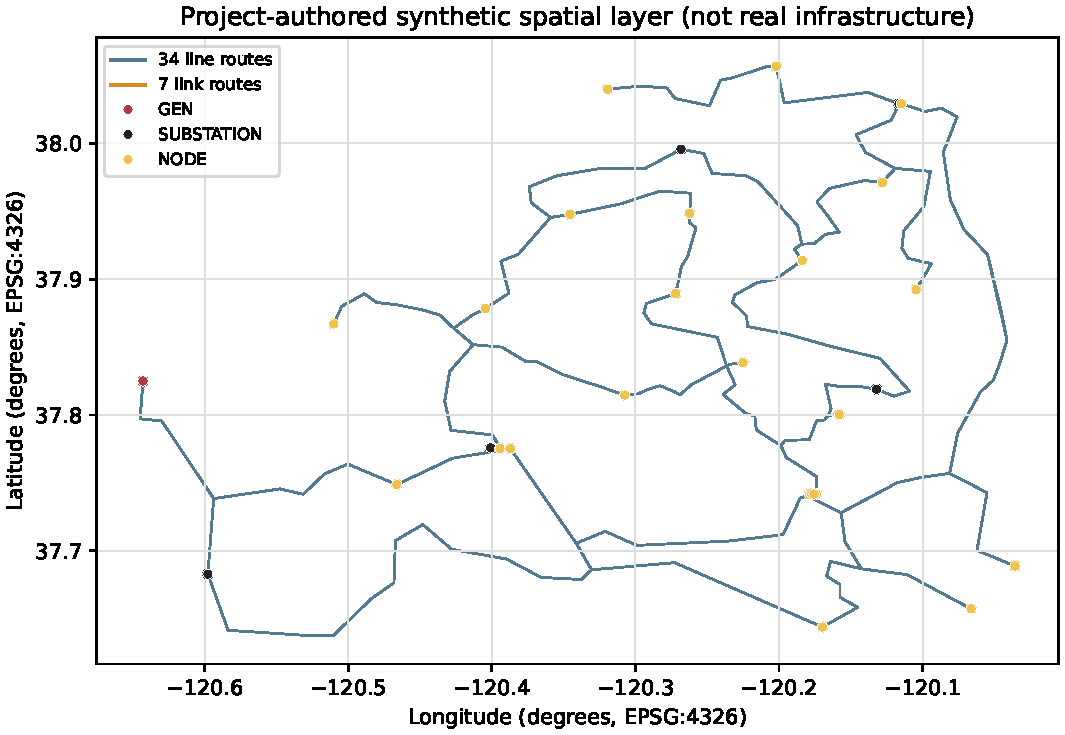
\includegraphics[width=\columnwidth]{figures/spatial-layer-map.pdf}
\caption{Project-authored synthetic bus points and branch routes in stored WGS84 coordinates. The figure is a dataset depiction, not a map of utility infrastructure.}
\label{fig:map}
\end{figure}

\section{Reproducible Construction and Validation}
\subsection{Construction workflow}
A project script constructs the canonical layer from a frozen, documented input reference, reconciles route orientation to the declared \texttt{fbus}$\rightarrow$\texttt{tbus} direction, and adds the public identifier and branch-type fields. A documented correction resolves a branch-24 source-label inconsistency. The workflow snaps only source route endpoints within a declared 500-m construction threshold to their associated bus coordinates; this is a construction rule, not a measure of physical line accuracy.

The release archive is manifest-first. It includes the canonical GeoJSON, schema, provenance/readme material, validation code, selected tests, release manifest, and SHA-256 checksums. The deterministic builder updates member hashes before constructing the archive. Figure~\ref{fig:workflow} summarizes this traceable release path.

\begin{figure}[!t]
\centering
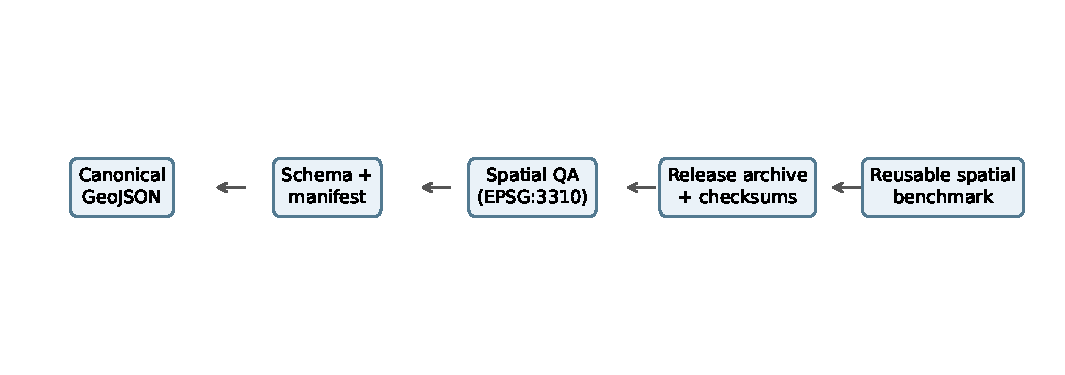
\includegraphics[width=\columnwidth]{figures/release-workflow.pdf}
\caption{Release workflow. Boxes represent artifacts and executed checks; the diagram does not represent a performance-evaluation pipeline.}
\label{fig:workflow}
\end{figure}

\subsection{Technical validation protocol}
The validation procedure operates on the released GeoJSON rather than on screenshots or manually copied values. It checks: (i) the 30/41 feature counts and stable-ID domains; (ii) allowed branch-type domains; (iii) JSON Schema conformance; (iv) valid, simple, nonzero-length LineStrings; (v) transformed endpoint distance from each route endpoint to the referenced bus point; (vi) graph connectivity induced by \texttt{fbus}/\texttt{tbus}; and (vii) metric route lengths after EPSG:4326-to-EPSG:3310 transformation with explicit longitude/latitude axis ordering.

Let $p_i$ be the projected coordinate of bus $i$ and $e_{ij}^{(s)}$, $e_{ij}^{(t)}$ be the projected start and end coordinates of route $(i,j)$. Endpoint reconciliation evaluates
\begin{equation}
 d_{ij}=\max\{\lVert e_{ij}^{(s)}-p_i\rVert_2,\lVert e_{ij}^{(t)}-p_j\rVert_2\},
\end{equation}
with acceptance criterion $\max d_{ij}\leq0.01$ m. Route length is computed as the planar length of each EPSG:3310-transformed LineString; it is not inferred from the source \texttt{length} or \texttt{Shape\_Length} attributes, whose units are undocumented.

\section{Executed Verification Evidence}
Table~\ref{tab:verification} reports the current executed pre-release evidence. These checks establish internal spatial and release integrity for this particular synthetic payload. They do not establish external geodetic accuracy, real-corridor fidelity, wildfire model validity, ACOPF validity, risk-prediction performance, or operational suitability.

\begin{table}[!t]
\caption{Executed pre-release verification evidence.}
\label{tab:verification}
\centering
\footnotesize
\begin{tabular}{p{0.47\columnwidth}p{0.45\columnwidth}}
\toprule
Check & Observed result \\
\midrule
Schema validation & 0 errors \\
Graph connectivity & One component containing all 30 buses \\
Route geometry & 0 invalid, non-simple, or zero-length routes \\
Endpoint alignment & Maximum 0.0 m; criterion $\leq$0.01 m \\
Metric route length & 687.388234 km total; EPSG:3310 \\
Automated test suite & 25 tests passed at the recorded pre-release build \\
Release-package validator & Passed; archive checksum recorded in repository \\
\bottomrule
\end{tabular}
\end{table}

The 687.388234-km total differs from the 702-km figure described for the prior case study \cite{sohrabi2024wildfire}. The release treats this as a disclosed spatial-layer difference, not as an error to be forced away and not as evidence of superiority. Any downstream analysis must report which geometry version and metric procedure it uses.

\section{Use, Limitations, and Release Requirements}
Appropriate uses include topology-aware GIS demonstrations, spatial-overlay methods, reproducible teaching examples, and interfaces for independently licensed wildfire, weather, fuel, or grid-analysis components. Users may replace compatible inputs or add method-specific attributes, provided they retain provenance, avoid reusing immutable IDs for altered features, and document changes.

The benchmark has important limits. It is synthetic. It contains neither terrain/fuel/weather data nor fire simulations; it does not validate wildfire spread, component exposure, dispatch, outages, power flow, or risk. Straight or source-derived route geometry should not be interpreted as surveyed corridors. The present GitHub release is public but pre-DOI. Before an archival release and manuscript submission, the project requires an independent cold-start reproduction, an external technical review, final author/funder/affiliation metadata, a release tag, an archived DOI, and a final provenance/rights review.

\section{Conclusion}
This work packages a narrow but useful research asset: a transparent, synthetic georeferencing of the IEEE 30-bus topology with stable identifiers and executable spatial quality controls. Its evidence supports claims of internal spatial consistency and reproducible release packaging only. By keeping wildfire-grid modeling as an optional downstream use, the dataset can support a broader class of spatial-method studies while avoiding unsupported operational or physical claims. The next release stage is independent reproduction and archival publication, followed by revision of this draft against documented reviewer feedback.

\section*{Data and Code Availability}
The pre-release dataset, code, validation report, archive manifest, and tests are available at \url{https://github.com/BehrouzSohrabi/georeferenced-ieee30-wildfire-benchmark}. The release is not yet assigned a DOI. Third-party inputs are excluded or pointer-only as documented in the repository.

\section*{Acknowledgment}
To be completed after confirmation of contributors, institutional affiliations, funding, and independent reviewers.

\bibliographystyle{IEEEtran}
\bibliography{references}
\end{document}
